\documentclass[tikz,border=5pt]{standalone}
\usepackage[T1]{fontenc}
\usepackage{lmodern,amsmath,amssymb}
\usetikzlibrary{arrows.meta,calc,positioning,fit,backgrounds,shapes.geometric,matrix,decorations.pathreplacing,patterns}
\definecolor{ink}{gray}{0.08}
\definecolor{wash}{gray}{0.965}
\definecolor{soft}{gray}{0.45}
\tikzset{box/.style={draw=ink,line width=.65pt,fill=white,align=center,inner sep=4pt,outer sep=0pt,font=\small},flow/.style={draw=ink,line width=.65pt,-{Latex[length=1.8mm,width=1.3mm]},rounded corners=2pt},annotation/.style={font=\scriptsize,text=soft,align=center},groupbox/.style={draw=soft,dashed,line width=.45pt,fill=wash}}
\begin{document}
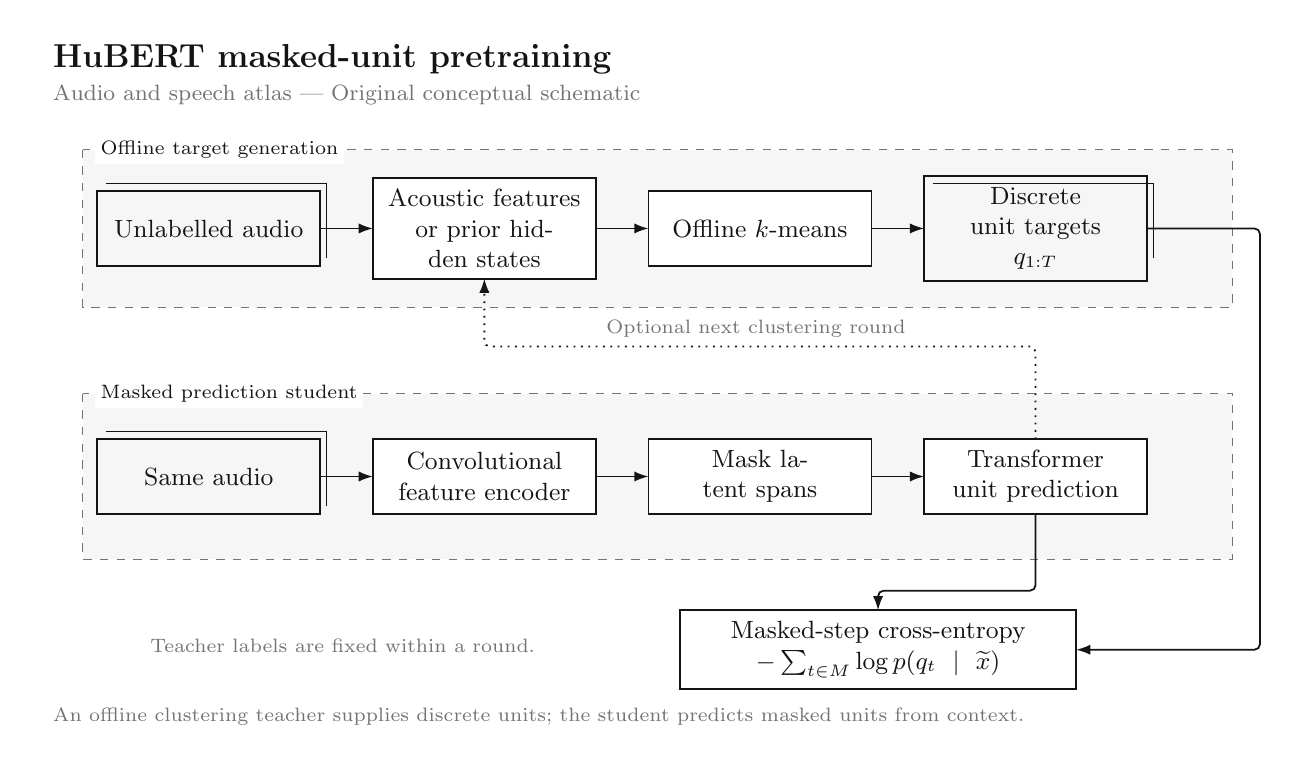
\begin{tikzpicture}[x=1cm,y=-1cm,font=\rmfamily,text=ink]

\path[use as bounding box] (0,0) rectangle (16,9);
\node[anchor=west,font=\large\bfseries] at (.2,.4) {HuBERT masked-unit pretraining};
\node[anchor=west,font=\footnotesize,text=soft] at (.2,.85) {Audio and speech atlas | Original conceptual schematic};
\begin{pgfonlayer}{background}
\draw[groupbox] (0.7,1.55) rectangle (15.299999999999999,3.55);
\node[anchor=west,font=\scriptsize,fill=white,inner sep=2pt] at (0.85,1.55) {Offline target generation};
\draw[groupbox] (0.7,4.65) rectangle (15.299999999999999,6.75);
\node[anchor=west,font=\scriptsize,fill=white,inner sep=2pt] at (0.85,4.65) {Masked prediction student};
\end{pgfonlayer}
\node[box,fill=wash,minimum width=2.8cm,minimum height=0.95cm,text width=2.55cm] (audioT) at (2.3,2.55) {Unlabelled audio};
\draw[ink,line width=.4pt] (0.9999999999999999,1.9749999999999996) -- (3.8,1.9749999999999996) -- (3.8,2.925);
\node[box,minimum width=2.8cm,minimum height=0.95cm,text width=2.55cm] (feat) at (5.8,2.55) {Acoustic features\\or prior hidden states};
\node[box,minimum width=2.8cm,minimum height=0.95cm,text width=2.55cm] (cluster) at (9.3,2.55) {Offline $k$-means};
\node[box,fill=wash,minimum width=2.8cm,minimum height=0.95cm,text width=2.55cm] (units) at (12.8,2.55) {Discrete unit targets\\$q_{1:T}$};
\draw[ink,line width=.4pt] (11.5,1.9749999999999996) -- (14.3,1.9749999999999996) -- (14.3,2.925);
\node[box,fill=wash,minimum width=2.8cm,minimum height=0.95cm,text width=2.55cm] (audioS) at (2.3,5.7) {Same audio};
\draw[ink,line width=.4pt] (0.9999999999999999,5.125000000000001) -- (3.8,5.125000000000001) -- (3.8,6.075);
\node[box,minimum width=2.8cm,minimum height=0.95cm,text width=2.55cm] (cnn) at (5.8,5.7) {Convolutional\\feature encoder};
\node[box,minimum width=2.8cm,minimum height=0.95cm,text width=2.55cm] (mask) at (9.3,5.7) {Mask latent spans};
\node[box,minimum width=2.8cm,minimum height=0.95cm,text width=2.55cm] (trans) at (12.8,5.7) {Transformer\\unit prediction};
\node[box,minimum width=5.0cm,minimum height=0.85cm,text width=4.75cm] (loss) at (10.8,7.9) {Masked-step cross-entropy\\$-\sum_{t\in M}\log p(q_t\mid \widetilde{x})$};
\begin{pgfonlayer}{background}
\draw[flow] (audioT.east) -- (feat.west);
\draw[flow] (feat.east) -- (cluster.west);
\draw[flow] (cluster.east) -- (units.west);
\draw[flow] (audioS.east) -- (cnn.west);
\draw[flow] (cnn.east) -- (mask.west);
\draw[flow] (mask.east) -- (trans.west);
\draw[flow] (trans.south) -- (12.8,7.15) -- (10.8,7.15) -- (loss.north);
\draw[flow] (units.east) -- (15.65,2.55) -- (15.65,7.9) -- (loss.east);
\draw[flow,dotted] (trans.north) -- (12.8,4.05) -- (5.8,4.05) -- (feat.south);
\end{pgfonlayer}
\node[align=center,anchor=center,font=\scriptsize,text=soft,text width=6cm] at (9.25,3.82) {Optional next clustering round};
\node[align=center,anchor=center,font=\scriptsize,text=soft,text width=5.6cm] at (4.0,7.85) {Teacher labels are fixed within a round.};
\node[anchor=west,align=left,font=\scriptsize,text=soft,text width=15.6cm] at (.2,8.75) {An offline clustering teacher supplies discrete units; the student predicts masked units from context.};
\end{tikzpicture}
\end{document}
